\section{Experimental Results}

To test our research question, an experiment was held using two EAs with different survivor selection methods, while the same initialization, mutation, crossover and parent selection operators were applied. The algorithms were tested in the EvoMan framework \cite{defranca2020evoman} against all eight enemies. Each EA was trained against two sets of enemies. The first set contains the enemies \textit{Flashman, Airman, Woodman,} and \textit{Heatman} and the second one the enemies \textit{Metalman, Crashman, Bubbleman,} and \textit{Quickman}.

In order to evaluate the two EAs, two types of plots were created. First, the line plots, displayed in Figure \ref{fig:lineplots}, depict the average of mean and maximum fitness of each generation and their standard deviation. Secondly, the box plots, shown in Figure \ref{fig:boxplots}, represent the individual gain of the best individual of each run tested 5 times against all 8 enemies for both algorithms split in the two training data sets. Moreover, we compared the performance difference of the algorithms with a t-test.

The line plots show an interesting picture of the two EAs for the different enemy groups. In the first line plot, it can be seen that EA1 has a lower maximum fitness, but a higher average fitness than EA2 for the first enemy group. Second, EA2 shows a higher variance than EA1. The second plot, with both algorithms being trained against enemy group 2, displays that EA1 shows higher fitness maximum and average than EA2. As in the first line plot, the standard deviation of EA2 is higher than for EA1. It has to be noted that the fitness already starts at a high level. This is due to the seeded initialization. 

\intextsep

\begin{figure}[H]%
	\centering
	\subfloat{{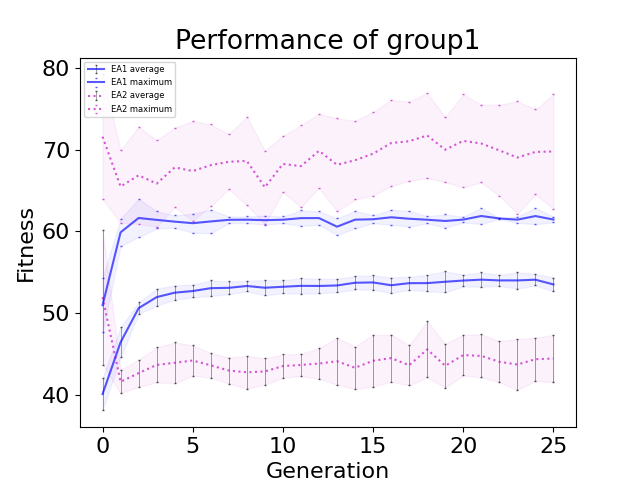
\includegraphics[scale=0.23]{Assets/Lineplot_Group1.png} }}%
	\qquad
	\subfloat{{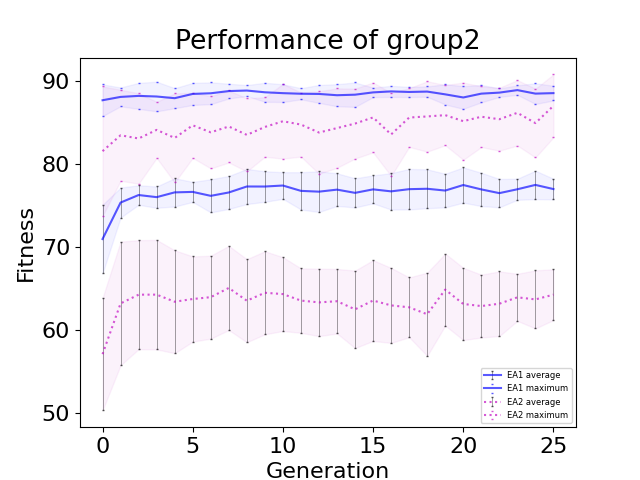
\includegraphics[scale=0.23]{Assets/Lineplot_Group2.png} }}%
	\caption{Line plots}
	\label{fig:lineplots}
\end{figure}

The box-plots represent the best individual of each run tested 5 times against all 8 enemies. In relevance with the line plots, the box-plots of the first training group show that EA2 has a higher average gain and variance compared to EA1. Moreover, for the second training group, the variance is lower and EA1 has higher gain and mean than EA1. The t-test emphasized that the EAs do not significantly differ from each other, with a \textit{p}-value of 0.97.



\intextsep

\begin{figure}[H]%
	\centering
	\subfloat{{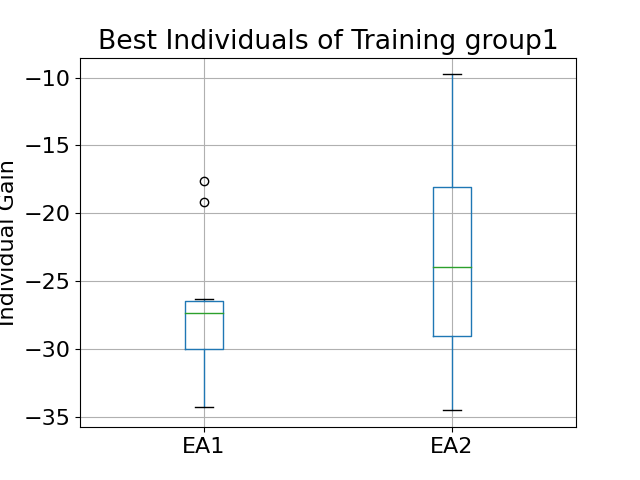
\includegraphics[scale=0.23]{Assets/Boxplot_Group1.png} }}%
	\qquad
	\subfloat{{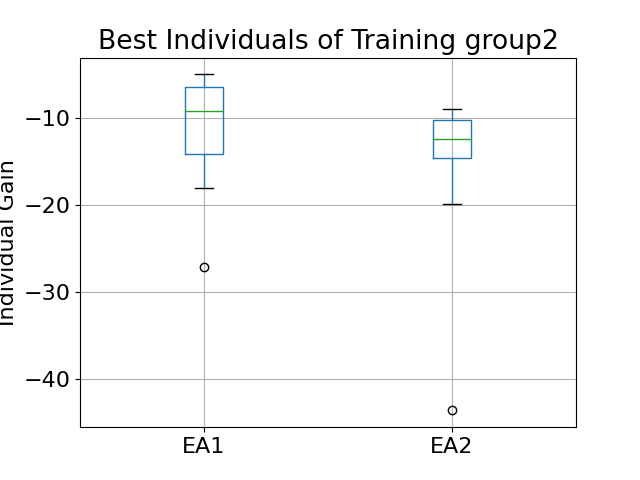
\includegraphics[scale=0.23]{Assets/Boxplot_Group2.png} }}%
	\caption{Box plots comparing the two groups}
	\label{fig:boxplots}
\end{figure}

The Table \ref{table:bestind} shows the average results of our best individual. The results show that the individual consistently wins against \textit{Airman, Metalman, Crashman,} \textit{Quickman}, and inconsistently against \textit{Bubbleman}.

\intextsep

\begin{table}[H]
\begin{center}
\scalebox{0.58}{
\begin{tabular}{||c | c | c ||} 
 \hline
 enemy & enemy life average & player life average \\ [0.5ex] 
 \hline\hline
 Flashman & 78 & 0  \\ 
 \hline
 Airman & 0 & 37.2  \\ 
 \hline
 Woodman & 58 & 0  \\ 
 \hline
 Heatman & 74 & 0  \\ 
 \hline
 Metalman & 0 & 42.16  \\ 
 \hline
 Crashman & 0 & 5.8  \\ 
 \hline
 Bubbleman & 20 & 25.6  \\ 
 \hline
 Quickman & 0 & 47.2  \\ 
 \hline
\end{tabular}
}
\end{center}
\bigskip
\caption{Average result of our best individual, over five runs.}
\label{table:bestind}
\end{table}


